\chapter{Prehľad algoritmov}\label{chap:algoritmy}

V tejto kapitole si spravíme prehľad algoritmov, ktoré existujú na nájdenie 
minimálnej dominujúcej množiny. Najprv zadefinujeme minimálnu dominujúcu 
množinu, neskôr určíme požiadavky na algoritmy a potom popíšeme jednotlivé 
konkrétne algoritmy.

\section{Dominujúce množiny}

\emph{Dominujúca množina} $S$ na grafe $G = (V, E)$ je podmnožina množiny 
vrcholov $V$ grafu $G$ taká, že každý vrchol grafu sa v množine nachádza 
alebo je susedný s dominujúcou množinou. Pre množinu platí: $N[S] = V$. 
Z definície je zrejmé, že o dominujúcich množinách má zmysel hovoriť iba pri 
grafoch s konečným počtom vrcholov.

\emph{Minimálna dominujúca množina} $S_M$ je dominujúca množina s najmenšou 
kardinalitou.

\emph{Dominančé číslo} $\gamma (G)$ grafu $G$ je kardinalita minimálnej 
dominujúcej množiny. Ak je množina $S_M$ minimálnou dominujúcou množinou, tak 
platí, že $\gamma (G) = |S_M|$.

Na tomto mieste zadefinujeme aj vrcholové pokrytie. Uvádzame ho tu preto, lebo 
problém nájdenia vrcholového pokrytia súvisí s problémom nájdenia minimálnej 
dominujúcej množiny. \emph{Vrcholové pokrytie} $S^\prime$ na grafe $G = (V, E)$ 
je podmnožina množiny vrcholov $V$ grafu $G$ taká, že každá hrana $xy \in E$ 
je incidentná s vrcholom vrcholového pokrytia. Pre množinu platí: 
$\forall xy \in E: x \in S^\prime \vee y \in S^\prime $

Podobne ako pri minimálnej dominujúcej množine, existuje aj minimálne vrcholové 
pokrytie.

Jedným zo spôsobov, ako vyriešiť problém nájdenia minimálnej dominujúcej 
množiny je previesť ho na problém množinového pokrytia. \emph{Množinové 
pokrytie} je súbor množín, ktorých zjednotenie obsahuje všetky prvky univerza. 
Formálne je daná usporiadaná dvojica $(\mathcal{S}, \mathcal{U})$, kde:

\begin{itemize}
	\item množina množín $\mathcal{S}$ obsahuje množiny $S_1, S_2, S_3, ..., 
		S_n$ také, že $\bigcup_{i = 1}^{n} S_i = \mathcal{U}$;
	\item množina $\mathcal{U}$ je množina všetkých prvkov a nazýva sa 
		\emph{univerzum}.
\end{itemize}

Množinové pokrytie je podmnožina $\mathcal{C} \subseteq \mathcal{S}$ množín, 
pre ktorú platí, že $\bigcup_{C \in \mathcal{C}} C = \mathcal{U}$.

\section{Požiadavky na algoritmy}

Táto práca ma za úlohu nájsť vhodný algoritmus na hľadanie minimálnej 
dominujúcej množiny. Ale pre reálne dáta. To znamená, že grafy, na ktorých 
budeme minimálnu dominujúcu množinu hľadať majú veľa vrcholov. Avšak problém 
nájdenia minimálnej dominujúcej množiny na grafe sa dá redukovať na problém 
vrcholového pokrytia, o ktorom vieme, že je NP-ťažký. To znamená, že na 
vyrátanie minimálnej dominujúcej množiny treba veľmi veľa výpočtového času na 
súčasných počítačoch. Keďže pre reálne požiadavky je častokrát lepší nejaký, 
aj keď nie optimálny výsledok, tak sme sa rozhodli, že algoritmus nemusí dávať 
optimálny výsledok, ale môže dať približný výsledok v rozumnom čase. Rozumný 
čas však neurčujeme absolútne, keďže počítače sa vyvíjajú a výpočtová sila sa 
zväčšuje, ale relatívne vzhľadom na ostatné algoritmy.

\subsection{Výhoda sieti malého sveta}

V tejto časti ukážeme dôkaz, že v sieťach malého sveta je počet hrán rádovo 
rovnaký ako počet vrcholov. A teda siete malého sveta sú riedke grafy. 

Budeme vychádzať z toho, že pre distribúciu stupňov vrcholov platí:
$$p(d) = kd^{-a} + q, 2 \leq a \leq 3$$

Pre dostatočne veľké siete môžeme nespojitú funkciu $p : \mnn \leftarrow \mnn$ 
aproximovať spojitou verziou $p : \mnr \leftarrow \mnr$. Ďalej o $q$ vieme, že 
$q \leq 1/V$, kde $V$ je počet vrcholov grafu. Pre počet hrán v grafe 
$G = (V, E)$ platí, že je to polovica súčtu stupňov grafu. Teda môžeme napísať, 
že: $$|E| = \frac{1}{2}\sum_{d = 1}^{\Delta(G)} p(d) \sim 
\frac{1}{2}\int_1^{\Delta (G)} \! p(x) \, \mathrm{d}x$$

Úpravou integrálu dostaneme:

\begin{align*}
\frac{1}{2}\int_1^{\Delta (G)} \! p(x) \, \mathrm{d}x \
&= \frac{1}{2}\int_1^{\Delta (G)} \! kd^{-a} + q \, \mathrm{d}x \\
&= \frac{1}{2}\left[\frac{1}{a - 1} \left(- k x^{- a + 1} + q x \
\left(a - 1\right)\right)\right]_1^{|V|}
\end{align*}

Keďže $2 \leq a \leq 3$ a integrujeme medzi $1$ a $\Delta (G)$, tak môžeme 
ohraničiť výpočet:

\begin{align*}
\frac{1}{2}\left[\frac{1}{a - 1} \left(- k x^{- a + 1} + q x \
\left(a - 1\right)\right)\right]_1^{\Delta (G)} \leq \
\frac{1}{2}\left[- \left( k x^{- 1} - q x \right)\right]_1^{\Delta (G)}
\end{align*}

Pre konštantu $q$ platí, že $q \leq \frac{1}{\Delta (G)}$. Inak by súčet v 
distribúcií bol väčší ako počet vrcholov.

\begin{align*}
\frac{1}{2}\left[- \left( k x^{- 1} - q x \right)\right]_1^{\Delta (G)} \leq \
\frac{1}{2}\left[- \left( k x^{- 1} - \
\frac{x}{\Delta (G)} \right)\right]_1^{\Delta (G)} 
\end{align*}

Ďalšou úpravou dostaneme:

\begin{align*}
\frac{1}{2}\left[- \left( k x^{- 1} - \frac{x}{\Delta (G)} \
\right)\right]_1^{\Delta (G)} \
\!\!\!\!&= \frac{1}{2}\left\{\left[- \left( k \Delta (G)^{- 1} - \
\frac{\Delta (G)}{\Delta (G)}\right)\right] - \
\left[- \left( k 1^{- 1} - \frac{1}{\Delta (G)}\right)\right] \right\}\\
&= \frac{1}{2}\left\{\left[- \left( k \Delta (G)^{- 1} - 1 \right)\right] - \
\left[- \left( k - \frac{1}{\Delta (G)} \right)\right] \right\} \\
&= \frac{1}{2}\left\{\left(k + 1\right) - \frac{k+1}{\Delta (G)} \right\}\\
&= \frac{1}{2}\left(k + 1\right)\left( 1 - \frac{1}{\Delta (G)} \right)\\
\end{align*}

Konštanta $k$ nemôže byť väčšia ako $|V|$. Inak by vrcholov stupňa 1 bolo viac 
ako vrcholov v grafe. Triviálne platí, že $\Delta (G) \leq |V|$. Takže 
odhad môžeme ďalej upraviť:
\begin{align*}
\frac{1}{2}\left(k + 1\right)\left( 1 - \frac{1}{\Delta (G)} \right)\
&=\frac{1}{2}\left(|V| + 1\right)\left( 1 - \frac{1}{|V|} \right)
\end{align*}

Takže platí, že:
\begin{align*}
|E|&\sim \frac{1}{2}\left(|V| + 1\right)\left( 1 - \frac{1}{|V|} \right)
\end{align*}
a teda aj, že počet hrán je $O(V)$.

Táto vlastnosť sietí malého sveta nám pomôže najmä pri voľnejšom výbere 
heuristík a pravidiel v algoritmoch uvedených ďalej. Keďže algoritmy vo 
všeobecnosti neuvažujú s týmto faktom, dáva nám možnosť vytvoriť zložitejší a 
stále rovnako efektívny algoritmus.

\subsection{Test, či je množina dominujúcou}

Keďže graf máme reprezentovaný susednosťou vrcholov, tak priamočiary algoritmus 
na zistenie, či je množina dominujúcou vyzerá následovne:

\begin{enumerate}
	\item Pre každý vrchol testovanej množiny pridaj do výslednej množiny 
všetkých susedov vrchola;
	\item porovnaj výslednú množinu s množinou vrcholov grafu.
\end{enumerate}

Nech má graf $n$ vrcholov, $m$ hrán a testovaná množina $s \leq n$ vrcholov. 
Potom v prvom kroku vykonáme $O(sm)$ operácií a v druhom $O(n^2)$ operácií. 
Test teda trvá $O(sm + n^2)$ operácií. Keďže počet vrcholov v testovanej 
množine môže byť rovnaký ako počet vrcholov grafu, tak odhad môžeme upraviť na 
$O(nm + n^2)$. Keďže pre siete malého sveta platí $O(m) = O(n)$, tak časový 
odhad pre siete malého sveta je $O(n^2)$.

\section{Skúšanie všetkých možností}

Prvým algoritmom, ktorý je v prehľade, je najzákladnejší algoritmu vyskúšania 
všetkých možností. Tento algoritmus budeme volať aj \emph{naivný}. Algoritmus 
vždy poskytne správny výsledok, ale výpočet bude trvať dlho. Je 
to však dobrý začiatok k ďalším algoritmom. Pracuje podľa krokov:

\begin{enumerate}
	\item \label{itm:bf:one} Vyber podmnožinu grafu;
	\item \label{itm:bf:two} otestuj, či je podmnožina dominujúcou množinou;
	\item \label{itm:bf:three} ak je podmnožina dominujúcou množinou a zároveň má najmenšiu 
kardinalitu, zapamätaj si ju;
	\item \label{itm:bf:four} opakuj, kým nevyberieš všetky možné podmnožiny práve raz;
	\item \label{itm:bf:five} jednou z minimálnych dominujúcich množín je zapamätaná množina a 
dominančné číslo grafu je jej kardinalita.
\end{enumerate}

Algoritmus je pomalý hlavne kvôli kroku \ref{itm:bf:four} -- všetkých možných 
podmnožín je $2^n$, takže výsledný algoritmus skúšania všetkých možností bude 
$\Omega (2^n)$. Súčasné počítače zvládnu úlohu v rozumnom čase vyrátať pre 
$n\le 40$.

Tam, kde je najväčšia slabina, je zväčša aj najväčší priestor na zlepšenie. 
Existujú mnohé zlepšenia, ktoré zrýchlia algoritmus nielen v priemernom 
(resp.~reálnom) prípade, ale aj zlepšia teoretický odhad.

\section{Heuristiky pre algoritmus skúšania všetkých možností}

V tejto sekcii si povieme niečo o možných heuristikách pre naivný algoritmus. 
\emph{Heuristika} v algoritme je nejaký prvok, zväčša zo skúsenosti z reálneho 
sveta, o ktorom predpokladáme, že nám pomôže zrýchliť výpočet. Aj keď obvykle 
nezlepšuje asymptotickú zložitosť, heuristiky sa snažia byť navrhnuté tak, aby 
vo väčšine prípad zrýchlili beh algoritmu.

Častým príkladom a aplikáciou je jedna z heuristík na hľadanie najkratšej 
cesty. Možná heuristika je, že prehľadávanie bude uprednostňovať cesty 
smerujúce k hľadanému bodu. Tu si všimnime, že pri heuristike potrebujeme 
poznať informáciu, ako je daná voľba dobrá. Pokiaľ nie je medzi hľadaným bodom 
a bodom, z ktorého hľadáme prekážka, algoritmus prehľadá oveľa menej hrán, 
ako pri bežnom prehľadávaní. Samozrejme, pokiaľ sme v bludisku a najkratšia 
cesta vedie "opačným" smerom, tak prehľadáme všetky hrany, kým sa dostaneme k 
cieľu.

Podobne je to aj pri hľadaní minimálnej dominujúcej množiny. Dobrým odhadom sa 
javí možnosť vybrať do potenciálnej množiny $S$ ten vrchol $v$, ktorý vie 
pokryť čo najviac vrcholov, teda sa javí byť čo najbližšie k cieľu. Čiže hľadáme 
$\argmax_v \left|N\left[S \cup {v}\right]\right|$ pre $v \in V$. Spojenie 
tejto heuristiky s vedomosťou, že siete malého sveta majú veľa klastrov ešte 
upevňuje predpoklad, že táto heuristika bude dávať na sieťach malého sveta 
rýchlejšie výsledky a "zlých" prípadov bude málo.

V pôvodnom algoritme, ktorý skúša všetky možnosti to znamená, že si pamätáme 
dočasný najlepší výsledok a neskúšame tie možnosti, ktoré obsahujú viac vrcholov 
ako dočasný najlepší výsledok. Samotné vynechanie tých možností, ktoré majú viac 
prvkov ako momentálny najlepší výsledok je veľké zrýchlenie, keďže pre súvislý 
graf s $N$ vrcholmi platí, že veľkosť minimálnej dominujúcej množiny je nanajvýš 
${N}\!/{2}$.

\section{Prevedenie na problém množinového pokrytia}

Ďalšou možnosťou, ako presne nájsť minimálnu dominujúcu množinu je previesť 
problém na problém množinového pokrytia, vyriešiť ten a výsledok opäť previesť.
Tento spôsob navrhol \citet{grandoni04} vo svojej dizertačnej práci. Dôvodom 
prevodu je fakt, že problém množinového pokrytia bol v minulosti oveľa 
skúmanejším problémom.
Keďže pri exponenciálnych algoritmoch celkom záleží aj na konštante pri 
exponente, odhad tohto algoritmu spresnil \citet{fomin05}. 

\citet{grandoni04} previedol problém minimálnej dominujúcej množiny na 
hľadanie minimálneho množinového pokrytia na grafe $G := (V, E)$ tak, že 
množiny predstavovali vrchol a jeho susedov. Univerzom je množina vrcholov 
grafu. Takže vytvoril usporiadanú dvojicu $({N[v] : v \in V }, V)$, čo je 
vstupný údaj pre hľadanie množinového pokrytia.

\subsection{Pomocné tvrdenia}

V algoritme využijeme následujúce tvrdenia, ktoré platia v každej dvojici 
$(\mathcal{S}, \mathcal{U})$ problému množinového pokrytia:
\begin{enumerate}
	\item pre každé dve navzájom odlišné množiny $S$ a $R$ také, že 
		$S, R \in \mathcal{S}, S \subseteq R$, platí, že existuje vrcholové 
		pokrytie, ktoré neobsahuje $S$;
	\item ak existuje prvok $u \in U$, ktorý patrí iba do jednej množiny 
		$S \in \mathcal{S}$, tak táto množina $S$ patrí do každého vrcholového 
		pokrytia.
\end{enumerate}

Zaujímavým pozorovaním je, že každá podmnožina s kardinalitou jeden, spĺňa 
práve jedno z tvrdení.

V prípade, že všetky podmnožiny $S \in \mathcal{S}$ sú dvojprvkové, problém 
sa dá redukovať na hľadanie maximálneho párenia. \emph{Párenie} v grafe $G$ 
je množina hrán $M$ taká, že hrany nemajú spoločný ani jeden vrchol. 
\emph{Maximálne párenie} je párenie s najväčšou mohutnosťou.

Z inštancie problému množinového pokrytia $(\mathcal{S}, \mathcal{U})$, kde 
$|S| = 2, S \in \mathcal{S}$, vieme spraviť graf $G^\prime = (V, E)$ tak, 
že množinou vrcholov bude množina univerza, čiže $V = \mathcal{U}$ a množinu 
hrán $E$ budú tvoriť podmnožiny $S \in \mathcal{U}$. Minimálnu dominujúcu 
množinu na grafe reprezentovanú dvojicou $(\mathcal{S}, \mathcal{U})$ vieme 
určiť pomocou minimálneho hranového pokrytia na grafe $G^\prime$. 
Minimálne hranové pokrytie zase vieme získať pomocou maximálneho párenia. 
Keďže hranám v grafe $G^\prime$ zodpovedá práve jedna podmnožina 
$S \in \mathcal{S}$ v dvojici $(\mathcal{S}, \mathcal{U})$, tak vieme určiť 
maximálne množinové pokrytie.

\subsection{Algoritmus}

Samotný algoritmus hľadania minimálneho množinového pokrytia je založený na 
princípe rozdeľuj a panuj. Pracujeme s inštanciou $(\mathcal{S}, \mathcal{U})$. 
Jeho triviálny prípad je, keď $|\mathcal{S}| = 0$. Pred rozdelením sa snaží 
odstrániť podmnožiny kardinality $1$.  Ak majú všetky podmnožiny mohutnosť 
práve dva, problém sa prevedie na problém maximálneho párenia. Ak má nejaká 
množina kardinalitu väčšiu ako 2 nastáva delenie. Spájanie výsledkov spočíva 
iba v porovnaní, ktorá z vetiev dala lepší výsledok. Výstupom algoritmu je 
množina podmnožín, ktorá tvorím minimálne množinové pokrytie. Algoritmus 
dostáva za vstup iba množinu podmnožín $\mathcal{S}$ a vyzerá následovne 
(v algoritme sú kvôli prehľadnosti podmnožiny nazývané množinami):

\begin{enumerate}
	\item ak je množina množín $\mathcal{S}$ prázdna, vráť prázdnu množinu;
	\item ak je nejaká množina $R$ podmnožinou inej množiny $S$, vráť výsledok 
		algoritmu pre $\mathcal{S} \setminus R$;
	\item ak existuje jedinečný prvok medzi množinami a ten je obsiahnutý (iba) 
		v množine $R$, vráť výsledok algoritmu pre $\mathcal{S} \setminus R$ 
		zjednotený s množinou $R$;
	\item ak majú všetky množiny mohutnosť dva, tak vráť výsledok z maximálneho 
		párenia;
	\item inak spusti dvakrát algoritmus s vynechaním ľubovoľnej množiny $R$; 
		raz ju vynechaj s množiny množín $\mathcal{S}$, vtedy sa do výsledku 
		nezaráta; druhý raz odstráň zo všetkých množín prvky množiny $R$ a 
		zarátaj množinu do výsledku; porovnaj, pre ktoré spustenie dal 
		algoritmus lepší výsledok a ten vráť.
\end{enumerate}

Ako vidno, krok 1 je triviálny prípad. Kroky 2, 3 a 4 sú popísané vyššie. 
V kroku 5 je slovo ľubovoľný. Toto správanie sa dá zameniť pomocou nejakej 
heuristiky. Prirodzene sa núka skúsiť vyberať množiny s najväčšou mohutnosťou 
najskôr, keďže tie redukujú ostatné množiny najviac.

\section{Pažravý algoritmus}\label{sec:greedy}

V predchádzajúcich častiach sme si popísali algoritmy, ktoré rátajú presné 
výsledky. Na veľkých sieťach, napríklad na zobrazeniach skutočných sietí, 
sú však nepoužiteľné. Preto si musíme vystačiť iba s približným výsledkom. 

Prvým algoritmom, ktorý uvedieme a bude výsledok určovať iba približne, bude 
jednoduchý pažravý algoritmus, od ktorého si postupne odvodíme iné a použijeme 
viacero postupov, na riešenie problému nájdenia minimálnej dominujúcej množiny. 
Pre pripomenutie -- \emph{pokrytie vrchola} je množina všetkých jeho susedov 
vrátane vrchola a \emph{pokrytie množiny} je prienik pokrytie vrcholov množiny. 

Algoritmus vyzerá následovne:
\begin{enumerate}
	\item na začiatku je výsledná množina prázdna;
	\item do výslednej množiny pridaj vrchol, ktorý pokryje čo najviac ešte 
		nepokrytých vrcholov;
	\item opakuj predošlý bod, až kým nebude výsledná množina pokrývať všetky 
		vrcholy;
	\item vráť výslednú množinu.
\end{enumerate}

Za zmienku stojí, že v bode 3 algoritmus musí určiť, či výsledná množina už 
pokrýva všetky vrcholy. Toto z tohto algoritmu a jeho variantov robí algoritmy, 
ktoré sú zložité najmenej kvadraticky od počtu vrcholov.

Ako aj pri algoritmoch s exaktnými výsledkami, aj tu môžeme použiť nejaké 
heuristiky na druhý krok. O tých si povieme neskôr.

\section{Distribuovaný algoritmus}\label{sec:dist}

V tejto časti si ukážeme prerobenie pažravého algoritmu na distribuovaný, ktorý 
navrhol \citet{chapS}. 
Využijeme pri tom jedno pozorovanie. V bode 2 sa vyberie vrchol, ktorý pokrýva 
čo najviac ešte nepokrytých vrcholov. Počet ešte nepokrytých vrcholov môže 
ovplyvniť iba výber vrcholov zo vzdialenosti najviac 2. Preto, ak vrchol môže 
pokryť najviac vrcholov s pomedzi vrcholov vzdialených najviac 2, tak sa tento 
vrchol môže vybrať do výslednej množiny pred ostatnými. 

Toto pozorovanie vedie ku konštrukcii veľmi jednoduchého algoritmu (v každom 
vrchole):

\begin{enumerate}
	\item pre svoj vrchol vypočítaj počet ešte nepokrytých vrcholov;
	\item tento počet pošli algoritmom vo vrcholoch najviac vzdialených dve 
		hrany;
	\item ak vrchol pokrýva najväčší počet vrcholov vo vzdialenosti najviac 
		dva, tak vrchol pridaj do dominujúcej množiny (ak je takých vrcholov 
		viac, rozhodni náhodne -- napríklad podľa ID);
	\item opakuj od bodu 1, až kým vrchol nebude mať všetkých susedov 
		pokrytých;
\end{enumerate}

Tento algoritmus teoreticky funguje veľmi dobre. Počet vykonaných krokov bude 
lineárne úmerný počtu vrcholov grafu, keďže v každom kroku sa aspoň jeden 
vrchol vyberie. V skutočnosti má okrem veľa implementačných problémov uvedených 
v kapitole \ref{chap:vysledky} aj zlý počet krokov výpočtu pre niektoré typy 
grafov.

\begin{figure}
	\centering
	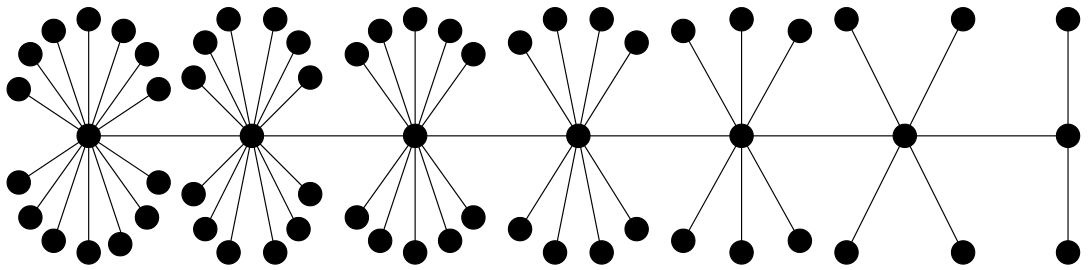
\includegraphics[width=1.0\textwidth]{obrazky/zle1}
	\caption{\emph{Graf, na ktorom beží distribuovaný algoritmus pomaly.} 
		Algoritmus v takejto situácií vyberá vrcholy postupne zľava doprava 
		a v každom kroku môže vybrať iba jeden vrchol.}
	\label{img:zle1}
\end{figure}

\begin{figure}
	\centering
	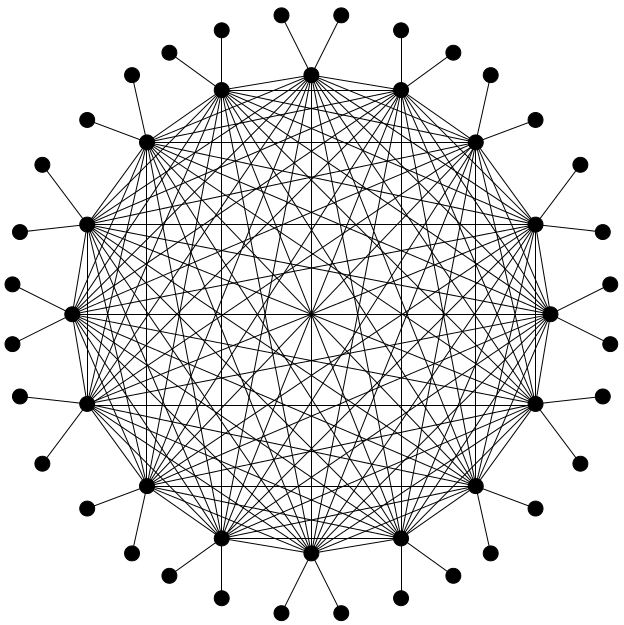
\includegraphics[width=0.5\textwidth]{obrazky/zle2}
	\caption{\emph{Graf, na ktorom beží distribuovaný algoritmus pomaly.} 
		Algoritmus v takejto situácií vyberá vrcholy náhodne, ale v každom 
		kroku iba jeden, pretože všetci potenciálny kandidáti sa blokujú.}
	\label{img:zle2}
\end{figure}

Na obrázku \ref{img:zle1} je vidieť jeden z možných grafov, na ktorom beží 
algoritmus pomaly. Algoritmus síce vyberie minimálnu dominujúcu množinu presne. 
Tá pozostáva z vrcholov na jej "osi". Ale v jednom opakovaní cyklu algoritmus 
vyberie najviac jeden vrchol, postupne zľava doprava. Je vidno, že algoritmus 
je $\Theta (N)$, kde $N$ je počet vrcholov grafu. Tento problém môžeme vyriešiť 
tak, že povolíme vybrať aj vrcholy s menším pokrytím vrchola. Tým síce 
zhoršíme aproximačný faktor, ale nie o veľa. Konkrétne, ak zhoršíme aproximačný 
faktor dvojnásobne, môžeme zaokrúhliť pokrytie vrchola na najbližšiu mocninu 
dvojky. Pri vyberaní najlepšieho kandidáta môžeme potom vybrať aj vrchol s 
menším pokrytím.

Druhou zlou možnosťou pre algoritmus je, keď je v grafe veľký klaster s 
vrcholmi rovnakého stupňa. Možnosť je znázornená na obrázku \ref{img:zle2}. 
Algoritmus nemôže naraz vybrať všetky vrcholy stupňa 3. Bráni mu v tom 
podmienka, že sa dá vybrať iba jeden z vrcholov spomedzi okolia vzdialenosti 
dva. Tu pomôže, ak povolíme vybrať viac vrcholov naraz, pokiaľ si príliš 
neprekážajú.

Algoritmus s týmito dvoma uvedenými vylepšeniami je zložitejší. Horným 
ohraničením pokrytia budeme nazývať najbližšiu hornú mocninu dvojky. Podobne, 
dolným ohraničením pokrytia budeme označovať najbližšiu dolnú mocninu dvojky.


\begin{enumerate}
	\item pre svoj vrchol vypočítaj počet ešte nepokrytých vrcholov;
	\item vypočítaj dolné ohraničenie pokrytia;
	\item zober dolné ohraničenia susedov vzdialených najviac 2;
	\item ak je dolné ohraničenie také, ako najväčšie dolné ohraničenie 
		spomedzi susedov, tak sa vrchol má šancu stať vybratým;
	\item táto šanca je nepriamo úmerná počtu vrcholov s najväčším dolným 
		pokrytím;
	\item vyber vrchol s pravdepodobnosťou vypočítanou vyššie;
	\item vypočítaj hodnotu $c$ -- počet kandidátov na vybratie spomedzi 
		pokrývajúcich vrcholov;
	\item ak je vrchol vybratý a súčet hodnôt $c$ pre pokrývajúce vrcholy 
		je menší alebo rovný ako trojnásobok počtu pokrývajúcich vrcholov, 
		tak vrchol pridaj do medzivýsledku;
	\item opakuj od bodu 1, až kým vrchol nebude mať všetkých susedov 
	pokrytých;
\end{enumerate}

Takto upravený algoritmus zvláda vypočítať dominujúce množiny o čosi 
rýchlejšie. Keďže množstvo klastrov a počet vrcholov s rovnakým stupňom je v 
sieťach malého sveta veľký, tak je predpoklad, že tento upravený algoritmus 
bude bežať oveľa rýchlejšie na sieťach malého sveta ako neupravený.

Vďalšej časti sa už nezaoberáme distribuovanými algoritmami ale jednoduchým 
pažravým algoritmom s rôznymi heuristikami.


\section{Heuristiky pre pažravý algoritmus}

V predchádzajúcich častiach sme zhrnuli rôzne postupy, ako riešiť problém 
minimálnej dominujúcej množiny. V tejto časti uvedieme heuristiky pre pažravý 
algoritmus spomenutý vyššie. Prvou heuristikou bude výber vrchola, ktorý 
pokrýva vrchol stupňa najviac jeden. Túto heuristiku rozvinieme a pridáme k 
nej ďalšie. Potom ich skombinujeme do rôznych algoritmov.

\subsection{Odstraňovanie výhonkov}

Prvá heuristikou, ktorú uvedieme je jednoduchá. V pažravom algoritme, pred tým, 
ako začneme vyberať vrcholy (krok 2), tak vyberieme všetky vrcholy stupňa nula 
a vrcholy, ktoré susedia s vrcholmi stupňa jeden (to znamená ich jediných 
susedov). Tieto vrcholy budeme nazývať \emph{výhonky}.


\subsection{Odstraňovanie kvetín}

Druhá heuristika spočíva v rozšírení prvej -- odstraňovaní výhonkov. Vo 
všeobecnosti sa dá povedať, že sme sa snažili vybrať vrchol s čo najväčším 
počtom nepokrytých susedov takých, ktoré majú všetkých susedov spoločných s 
vybratým vrcholom. Teda tvoria akýsi lokálny klaster "na okraji" grafu. 

Vrchol $v$, ktorý pokrýva $n$ vrcholov, ktoré majú za susedov iba susedov 
vrchola $v$, nazývame \emph{kvetinou} rádu $n$.

\subsection{Rozhodovanie rovnakých vrcholov}

Keď máme viacero rovnakých kandidátov (z pohľadu) na výber, je otázne, či si 
vybrať náhodný vrchol, vrchol s najmenším/najväčším ID alebo pridať nejaké 
pravidlo, ktoré rozhodne o priorite výberu. Tu si uvedieme nejaké pravidlá.

V základnom pažravom algoritme na hľadanie sietí malého sveta je často 
situácia, kde majú rovnaký počet ešte nepokrytých vrcholov vrcholy s úplne 
iným stupňom. Možno ešte podstatnejšia hodnota ako počet ešte nepokrytých 
susedov je počet vrcholov, ktoré po vybratí daného vrchola prestanú pokrývať 
akékoľvek vrcholy. Toto nie je to isté ako hľadanie kvetiny s najväčším rádom, 
lebo kvetiny sa vyskytujú iba na okrajoch grafu. Vrcholy vybraté takýmto 
rozhodovaním sa nachádzajú všade a preferujú susedov vzdialených 3 od už 
vybratých susedov (respektíve vzdialených 2 od pokrytých vrcholov). 

Treba si ale uvedomiť, že priemer siete malého sveta je malý a tak skutočná 
preferencia na "umiestnenie v grafe" nie je. Taktiež tento spôsob vyberania 
môže trochu korigovať "slepé" vyberanie vrcholov s väčšími stupňami.

\subsection{Výsledné algoritmy}

Vyššie uvedené heuristiky ide rôzne kombinovať a rôzne použiť. Na tomto mieste 
uvedieme algoritmus, ktorý skombinuje všetky pravidlá. Pre odstraňovanie 
výhonkov a odstraňovanie kvetín platí, že sa vykonajú iba raz -- na začiatku 
algoritmu. Po odstránení sa spustí pažravý algoritmus, ktorý vhodného kandidáta 
vyberie na základe pokrytia vrcholu a odstraňovania najvplyvnejších vrcholov.

Algoritmus vyzerá následovne:

\begin{enumerate}
	\item odstráň výhonky:
	\begin{enumerate}
		\item vyber vrcholy do výsledku;
		\item pokry susedov;
	\end{enumerate}
	\item postupne odstraňuj kvety (postupne preto, lebo z niektorý kvetov 
		prestanú byť kvety) -- kvety zotrieď podľa rádu a stupňa; potom 
		postupne, až kým nie je množina kvetov prázdna:
		\begin{enumerate}
			\item vyber kvet do výsledku;
			\item pokry susedov;
			\item odstráň tie kvety, ktoré už nie sú kvetmi;
		\end{enumerate}
	\item prepočítaj hodnoty pre "vplyvnosť" vrcholov;
	\item opakuj, až kým množina pokrytých vrcholov netvorí celý graf:
		\begin{enumerate}
			\item do výsledku vyber najlepšieho kandidáta podľa "vplyvnosti" 
				a stupňa;
			\item pokry susedov vybratého vrchola;
			\item prerátaj "vplyvnosť" susedov;
		\end{enumerate}
\end{enumerate}

Ide o upravený pažravý algoritmus. Upravený o heuristiky a pozorovania uvedené 
vyššie. Tento algoritmus sa dá rôzne modifikovať upravovaním heuristík a 
pravidiel. 

Ide o posledný uvedený algoritmus. V ďalších kapitolách sa venujeme 
implementačnej časti, rôznym testom a výsledkom.